\begin{longtable} { | c | p{12cm} | c | } 
\hline
	ID 	&	Issues	&		 Es. hours \\\hline
	58	&	Add icons to all buttons	&	1 hour	\\\hline
\caption{Issue ID 58}
\label{tab:spr4_iconstobuttons}
\end{longtable}

As the semester was coming to an end and we had to make the program costumer ready, we had to get rid of all the placeholders and add the real icons. The assignment itself was very trivial as it was a matter of changing all of the drawables. Furthermore we wanted to add text to each button as some of the icons were a bit too bland by themselves. As we added text we noticed pictures on buttons scales from width, so if we wanted the button to be quadratic, it was impossible to add text. We decided buttons were more appealing if had quadratic buttons and no text, than rectangular buttons with text. The differences are illustrated in figure \ref{fig:withoutIcons} and figure \ref{fig:withIcons}

\begin{figure} [h!]
\centering
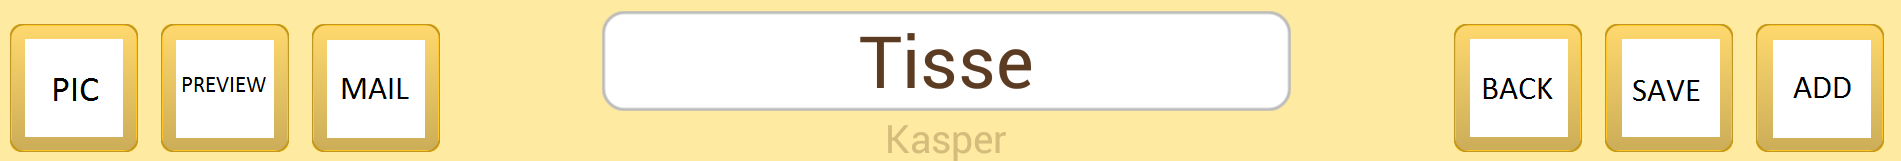
\includegraphics[width=0.9\textwidth]{Pics/Sprint4/topbarshit/withoutIcons.png}
\caption{This is the top bar before the addition of icons}
\label{fig:withoutIcons}
\end{figure}

\begin{figure} [h!]
\centering
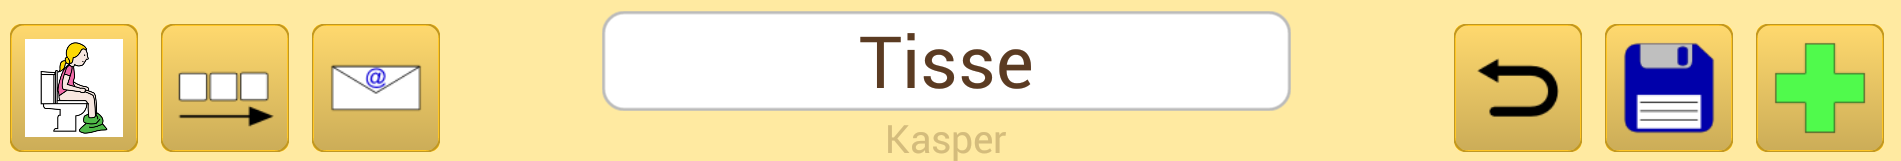
\includegraphics[width=0.9\textwidth]{Pics/Sprint4/topbarshit/withIcons.png}
\caption{This is the top bar after the addition of icons}
\label{fig:withIcons}
\end{figure}
